\documentclass{slide}

\usepackage{pgfpages}
\setbeameroption{show notes on second screen}

\title{Pipeline Architecture}
\subtitle{Software Architecture}
\author{Brae Webb}
\date{\week{2}}

\usepackage{languages}

\usepackage{tikz}
\usetikzlibrary{positioning}
\usetikzlibrary{arrows}
\usetikzlibrary{fit}

\begin{document}

\maketitle

\point[So far\dots]{Layered architectures reduce the impact of changing a layer}

%\note{We're emphasizing that pipeline architecture is a layered architecture taken to an extreme, minus the ability to have upward notifications.}

\questionanswer{Why does the layer order matter?\note{A consequence is layers have order.}}{Each layer implements a different interface.}

\point[So\dots]{If every layer implements the same interface?}

\note{We essentially have a pipeline architecture.}

\point[Extreme layered architecture]{Pipeline Architectures\footnote{sorta}}

\definition{Pipeline Architecture}{Components connected in such a way that the output of one component is the input of another.}

\questionanswer{Can you think of a \highlight{pipeline archiecture}?}{How about \highlight{bash}?}

\note[itemize]{
    \item Bash
    \item Compilers
    \item Functional programming
    \item ??
}

\begin{frame}[fragile]
\begin{code}[language=shell,mathescape]{}
$>>$ cat assignment.py | grep "hack" | wc -l | tee code-quality.txt
\end{code}
\only<2-3>{Notice:
\begin{itemize}
    \item Each program performs a small well-defined task.
    \item<3-> Each program implements the same interface (i.e. raw text).
\end{itemize}}
\only<4->{
    \centering
    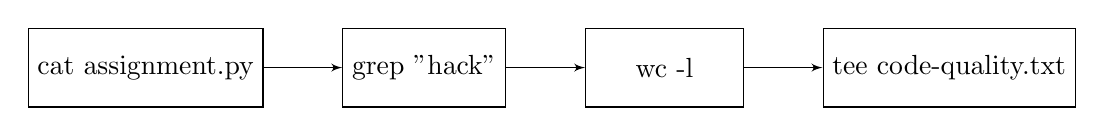
\begin{tikzpicture}[>=latex']
        \tikzset{block/.style= {draw, rectangle, align=center,minimum width=2cm,minimum height=1cm},}
    
        \node [block] (input) {cat assignment.py};
        \node [block, right =1cm of input] (grep) {grep "hack"};
        \node [block, right =1cm of grep] (wc) {wc -l};
        \node [block, right =1cm of wc] (tee) {tee code-quality.txt};
    
        \path[draw,->]
                    (input) edge (grep)
                    (grep) edge (wc)
                    (wc) edge (tee)
                    ;
    \end{tikzpicture}
}
\end{frame}

\begin{frame}[c]

\only<1->{{\large\par\bigskip
\begin{center}

\begin{tikzpicture}[>=latex']
    \tikzset{block/.style= {draw, rectangle, align=center,minimum width=2cm,minimum height=1cm},}

    \node [block] (filter1) {Filter};
    \node [block, right =2cm of filter1] (filter2) {Filter};
    \node [block, right =2cm of filter2] (filter3) {Filter};

    \path[draw,->]
                (filter1) edge node[above] {Pipe} (filter2)
                (filter2) edge node[above] {Pipe} (filter3)
                ;
\end{tikzpicture}
\end{center}
}
}

\note{Note the simplicity and modularity.}

\only<2->{
    \par\bigskip{\normalsize\color{primary}Filters}

    \huge Modular software components
}

\only<3->{
    \par\bigskip{\normalsize\color{primary}Pipes}

    \huge The flow of data between filters
}
\end{frame}

\begin{frame}{Types of Filters}
\begin{minipage}{0.45\textwidth}
\only<1->{
    \par\bigskip{\normalsize\color{primary}Producers}

    \huge Source of data
}

\only<2->{
    \par\bigskip{\normalsize\color{primary}Transformers}

    \huge Transform data
}
\end{minipage}
\begin{minipage}{0.45\textwidth}
\only<3->{
    \par\bigskip{\normalsize\color{primary}Testers}

    \huge Filter data
}

\only<4->{
    \par\bigskip{\normalsize\color{primary}Consumers}

    \huge Target for results
}
\end{minipage}
\end{frame}


\point[Exercise]{Label the bash pipeline}

\begin{frame}
\centering
\begin{tikzpicture}[>=latex']
    \tikzset{block/.style= {draw, rectangle, align=center,minimum width=2cm,minimum height=1cm},}

    \node [block,label=\only<2->{\only<2>{\color{focus}}Producer}] (input) {cat assignment.py};
    \node [block,label=\only<3->{\only<3>{\color{focus}}Tester}, right =1cm of input] (grep) {grep "hack"};
    \node [block,label=\only<4->{\only<4>{\color{focus}}Transformer}, right =1cm of grep] (wc) {wc -l};
    \node [block,label=\only<5->{\only<5>{\color{focus}}Consumer}, right =1cm of wc] (tee) {tee code-quality.txt};

    \path[draw,->]
                (input) edge (grep)
                (grep) edge (wc)
                (wc) edge (tee)
                ;
\end{tikzpicture}
\end{frame}

\definition{One Direction Principle}{Data should flow in one direction --- \highlight{downstream}.}

\note{This makes pipeline architectures bad for interactivity.}

\definition{Independent Filter Principle}{Filters should not rely on specific upstream or downstream components.}

\note[itemize]{
    \item This is not required but is strongly encouraged as it helps in designing good architectures.
    \item Note that producers and consumers can assume they don't have an upstream or downstream respectively.
}

\corollary{Generic Interface}{The interface between filters should be generic.}

\note{This follows from independent filters.}

\corollary{Composable Filters}{Filters (i.e. Transformers \& Testers) can be applied in any order.}

\note{This follows from independent filters.}

\note{The meaning of the process is determined by the designer who composes how filters are applied.}

\point[The Case Study]{Bash}

\note{Quick discussion about how the bash philosophy enables many small components which work well together.}

\begin{frame}
\centering
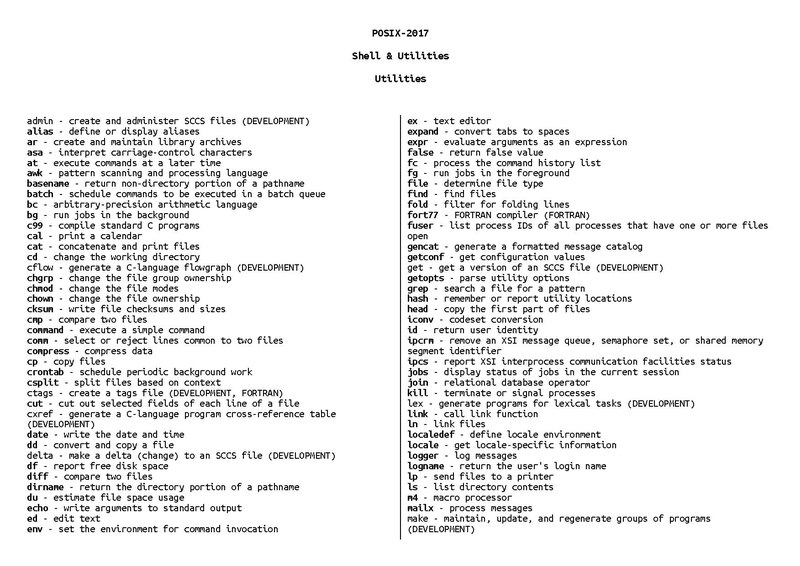
\includegraphics[width=0.9\textwidth]{bashcomponents.jpg}
\end{frame}

\question{Who has heard of \highlight{literate programming}?}

\note{We're now going on a quick tangent about how the pipeline archiecture of bash allowed McIlroy to best Knuth.}

\point[The Challenge --- set by Jon Bently]{
    \begin{enumerate}
        \item Read a file of text.
        \item Determine the n most frequently used words.
        \item Print out a sorted list of those words along with their frequencies.
    \end{enumerate}
}

\point[Knuth's Solution]{\highlight{17 pages} of elegant and descriptive code.}

\begin{frame}
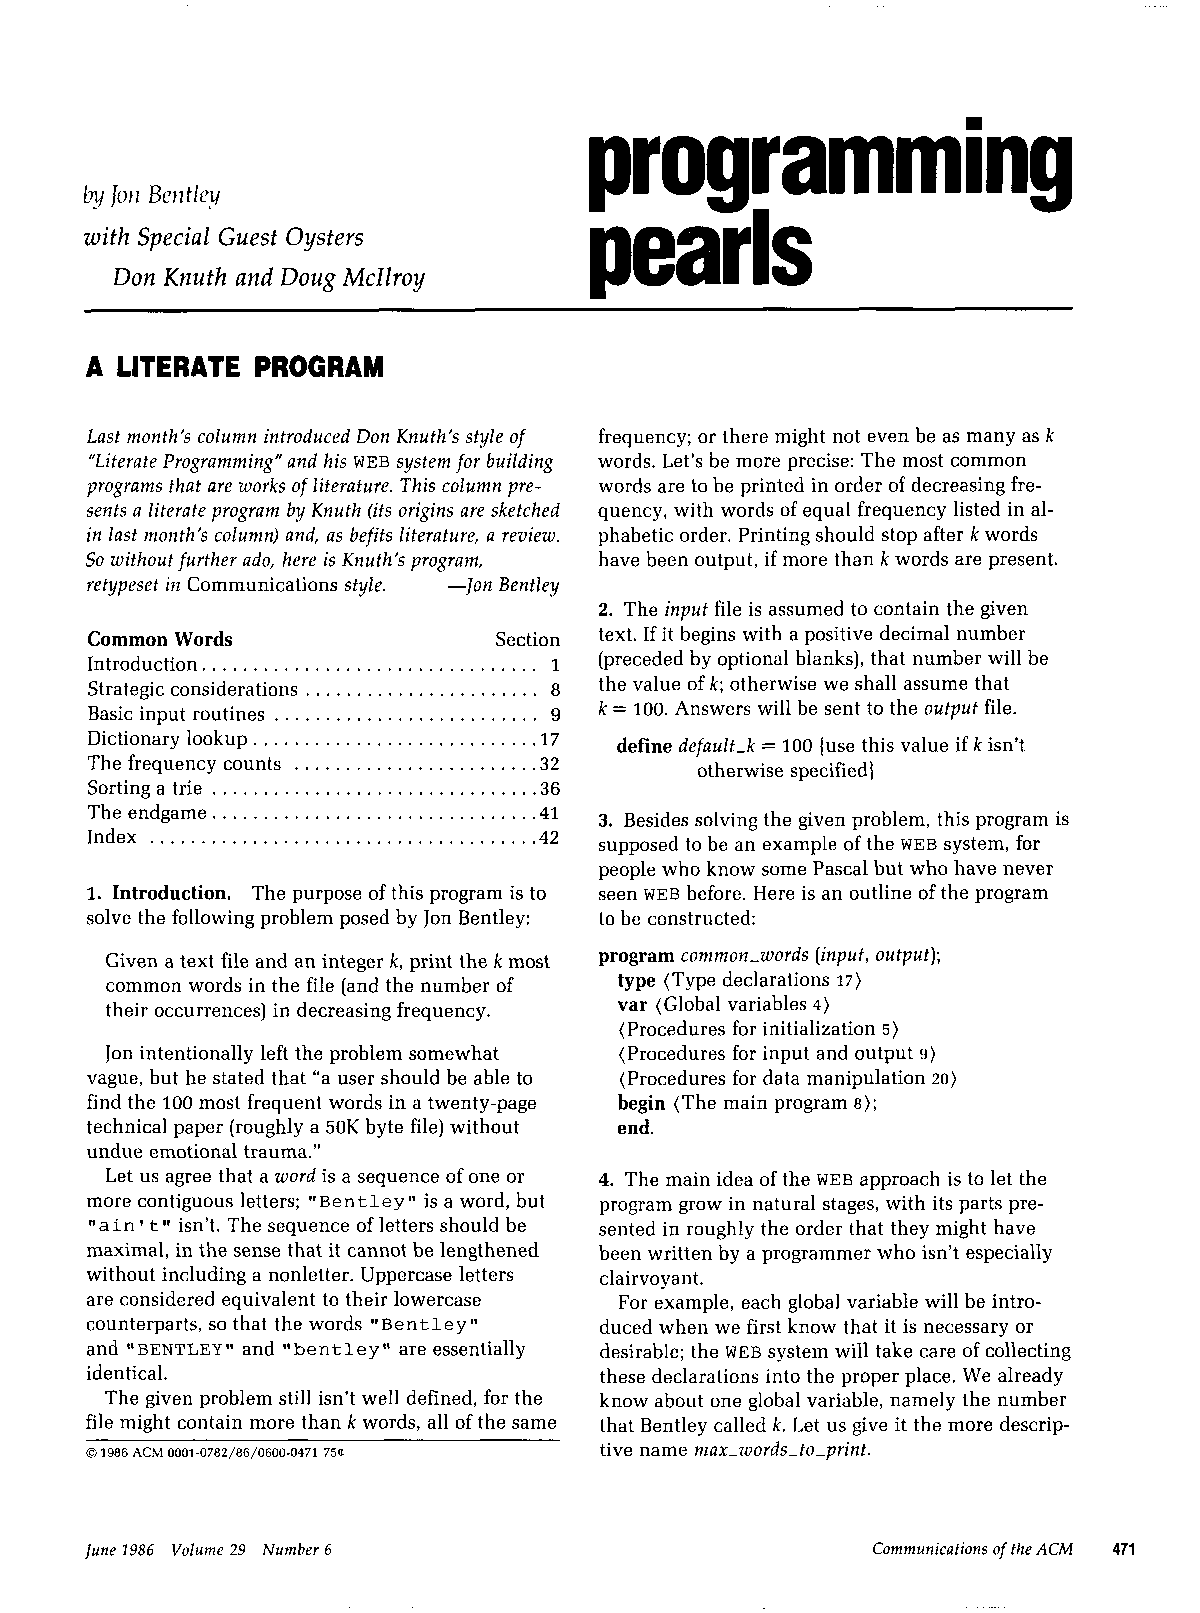
\includegraphics[page=1,width=0.45\textwidth]{perls.pdf}
\includegraphics[page=2,width=0.45\textwidth]{perls.pdf}
\end{frame}

\begin{frame}[fragile]
    \par\bigskip
        {\color{primary}McIlroy's Solution}
    \begin{code}[language=bash]{}
tr -cs A-Za-z '\n' | \
    tr A-Z a-z | \
    sort | \
    uniq -c | \
    sort -rn | \
    sed ${1}q
    \end{code}
\end{frame}

\note[enumerate]{
    \item Make one-word lines by transliterating the complement (-c) of the alphabet into newlines (note the quoted newline), and squeezing out (-s) multiple newlines. 
    \item Transliterate upper case to lower case.
    \item Sort to bring identical words together.
    \item Replace each run of duplicate words with a single representative and include a count (-c).
    \item Sort in reverse (-r) numeric (-n) order.
    \item Pass through a stream editor; quit (q) after printing the number of lines designated by the script’s first parameter (\${1})
}

\questionanswer{Is literate programming bad?}{No, the Unix philosophy is just good.}

\point[The Unix Philosophy]{
\begin{itemize}
\item Write programs that do one thing and do it well.
\item<2-> Write programs to work together.
\item<3-> Write programs to handle text streams, because that is a universal interface.
\end{itemize}}

\begin{frame}{Bash itself is a pipeline}
\centering
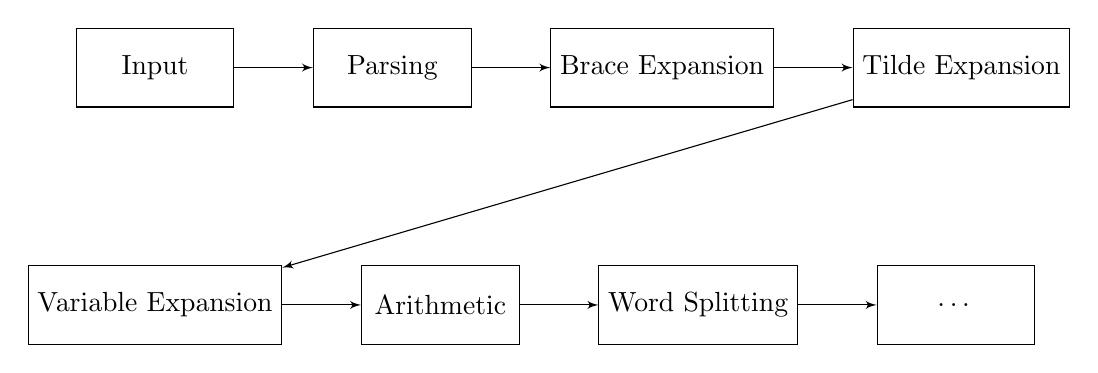
\begin{tikzpicture}[>=latex']
    \tikzset{block/.style= {draw, rectangle, align=center,minimum width=2cm,minimum height=1cm},}

    \node [block] (input) {Input};
    \node [block,right =1cm of input] (parsing) {Parsing};
    \node [block,right =1cm of parsing] (braces) {Brace Expansion};
    \node [block,right =1cm of braces] (tilde) {Tilde Expansion};
    \node [block,below =2cm of input] (variable) {Variable Expansion};
    \node [block,right =1cm of variable] (arithmetic) {Arithmetic};
    \node [block,right =1cm of arithmetic] (split) {Word Splitting};
    \node [block,right =1cm of split] (fin) {\dots};

    \path[draw,->]
                (input) edge (parsing)
                (parsing) edge (braces)
                (braces) edge (tilde)
                (tilde) edge (variable)
                (variable) edge (arithmetic)
                (arithmetic) edge (split)
                (split) edge (fin)
                ;
\end{tikzpicture}
\end{frame}

\note{Just an aside looking at it more practically rather than philosophically.}

%\point[Case Study]{Compilers}

%\note{Exploring how the pipeline architecture can be integrated with other architectural styles like blackboard.}

%\point[Case Study]{MapReduce}

%\note{Exploring the power in simplicity.}

%\questionanswer{What's the advantage of the map reduce pattern?}{Parallelism \cite{mapreduce}}

%\question{Using pipeline terminology, what filters do the \highlight{map} and \highlight{reduce} operators correspond to?}

\point[Reading...]{``Pipeline Architecture'' Notes \cite{pipeline-notes}}

\references{articles,books,ours}

\end{document}
